% Mirror: https://github.com/SIGma-UIUC/presentation-format
% --------------------------------------------------------------------
% This is a simple Beamer document that uses beamerthemesigma.sty
% Reading the comments should help you create a presentation even if
% you've never used Beamer before.
% --------------------------------------------------------------------

% Set our document class to Beamer
\documentclass[aspectratio=169]{beamer}

% Some packages for nice font encodings in the final PDF
\usepackage[utf8]{inputenc}
\usepackage[T1]{fontenc}

% From Jeff E
\usepackage{algo}

% Some more macros
\usepackage{sigmastyle}

% Citations
\usepackage{cite}

% To insert images
\usepackage{graphicx}

% Useful packages from the AMS
\usepackage{amsmath,amssymb,amsthm}

\usepackage{soul}

\usepackage{tikz}

% https://tex.stackexchange.com/questions/17522/pascals-triangle-in-tikz
\makeatletter
\newcommand\binomialCoefficient[2]{%
    % Store values 
    \c@pgf@counta=#1% n
    \c@pgf@countb=#2% k
    %
    % Take advantage of symmetry if k > n - k
    \c@pgf@countc=\c@pgf@counta%
    \advance\c@pgf@countc by-\c@pgf@countb%
    \ifnum\c@pgf@countb>\c@pgf@countc%
        \c@pgf@countb=\c@pgf@countc%
    \fi%
    %
    % Recursively compute the coefficients
    \c@pgf@countc=1% will hold the result
    \c@pgf@countd=0% counter
    \pgfmathloop% c -> c*(n-i)/(i+1) for i=0,...,k-1
        \ifnum\c@pgf@countd<\c@pgf@countb%
        \multiply\c@pgf@countc by\c@pgf@counta%
        \advance\c@pgf@counta by-1%
        \advance\c@pgf@countd by1%
        \divide\c@pgf@countc by\c@pgf@countd%
    \repeatpgfmathloop%
    \the\c@pgf@countc%
}
\makeatother



% Package for code highlighting
\usepackage{minted}
\setminted{linenos=true, breaklines=true, breakanywhere=true, style=default}
\usemintedstyle{monokai}

% Set a title
\title{Welcome to SIGma}

% Set a subtitle if you desire
\subtitle{}

% Whoever worked on the presentation:
\author{SIGma}

% A date, if you'd like.
\date{}

% An institute name, if you're so inclined
% \institute{University of Illinois Urbana-Champaign}

% Use the SIGma theme for this Beamer presentation
\usetheme{sigma}
% --------------------------------------------------------------------

% Begin document
\begin{document}

% Beamer calls each slide a "frame", defined within the environment:
% \begin{frame}
%   <frame content here>
% \end{frame}

% This frame is just the title.
\begin{frame}
\titlepage
\end{frame}

\begin{frame}{Outline}
  \tableofcontents
\end{frame}

\section{Officers in No Particular Order}

% Officer type people put info here
\begin{frame}{Anakin} 
        \begin{itemize}
        \item Math Major
        \item SIGPwny Crypto\footnotemark\ Gang + Admin team
        \item CA for CS 173 + CS 475
        \item Research with Sam
    \end{itemize}
    \footnotetext[1]{Not that one, the other one}
\end{frame}

\begin{frame}{Sam}
    \begin{itemize}
        \item Summer Amazon Intern
        \item CS Major
        \item Doing CS 374 Course Dev
        \item Doing Theory Research with Sariel Har-Peled
        \item Research with Anakin
    \end{itemize}
\end{frame}

\begin{frame}{Lou}
\begin{itemize}
    \item CS Major
    \item Current CS 225 CA (past CS 125 and 374 CA)
    \item Senior, selling soul to finance after this semester
\end{itemize}
\end{frame}

\begin{frame}{Aditya}
    \begin{itemize}
        \item ECE/Math double degree.
        \item Quantum error correction research w/Prof. Milenkovic.
        \item CA for ECE 391.
        \item Other interests: FP, PL, Crypto.
    \end{itemize} 
\end{frame}

\begin{frame}{Hassam}
    \begin{itemize}
        \item Intern at Amazon over the summer
        \item CS Major (takes math classes for fun ???)
        \item SIGPwny Crypto Gang + Admin team + Infra lead
        \item CA for CS 233, CS 173
        \item Compiler research
    \end{itemize}
\end{frame}

\begin{frame}{Phil}
    \begin{itemize}
        \item CS/Ling Major, Senior
        \item CA for CS 233
        \item SIGecom - game theory, economics, and computation
    \end{itemize}
\end{frame}

\section{Computing Fibonacci}
\frame{\sectionpage}

\begin{frame}{Recursive}
    \[
        F_n = \begin{cases}
                0                       & n = 0 \\
                1                       & n = 1 \\
                F_{n - 1} + F_{n - 2}   & n \geq 2
              \end{cases}
    \]
    
    \pause
    \vspace{20pt}
    \begin{table}[]
        \begin{tabular}{|c|c|c|c|c|c|c|c|c|c|c|c|c|c|}
            \hline
            $F_0$ & $F_1$ & $F_2$ & $F_3$ & $F_4$ & $F_5$ & $F_6$ & $F_7$ & $F_8$ & $F_9$ & $F_{10}$ & $F_{11}$ & $F_{12}$ & $F_{13}$ \\ \hline
            0     & 1     & 1     & 2     & 3     & 5     & 8     & 13    & 21    & 34    & 55       & 89       & 144      & 233      \\ \hline
        \end{tabular}
    \end{table}
\end{frame}

\begin{frame}{Recursive Computation}
    \begin{figure}
        \centering
        \includegraphics[scale=0.4]{images/F7_Recursion.png}
        \caption{From \cite{book:algorithms}}
    \end{figure}
\end{frame}

\begin{frame}{Can We Do Better?}
    We can use 12 multiplications to compute $x^{13}$ as follows: 
    \[
    x \to x^2 \to x^3 \to x^4 \to x^5 \to x^6 \to x^7 \to x^8 \to x^9 \to x^{10} \to x^{11} \to x^{12} \to x^{13}
    \]
    
    \pause
    
    But if we first compute powers as such
    \begin{align*}
        x^2 &\gets x \cdot x \\
        x^4 &\gets x^2 \cdot x^2 \\ 
        x^8 &\gets x^4 \cdot x^4 \\
    \end{align*}
    
    \pause
    
    Using these we compute $x^8 \cdot x^4 \cdot x^1 = x^{13}$ in just 5 total multiplications.
    
    \pause
    
    We can generalize this using binary
    \begin{table}[]
    \begin{tabular}{|l|l|l|l|}
    \hline
    \textbf{1} & \textbf{1} & \textbf{0}  & \textbf{1} \\ \hline
    $8$        & $4$        & $2$         & $1$        \\
    \hline
    \end{tabular}
    \end{table}
\end{frame}

\begin{frame}{Building an Algorithm}
    \[
        13 = 8 + 4 + 1 = \textbf{1101}_2
    \] \pause
    
    \begin{table}[]
        \centering
        \begin{tabular}{|l|c|c|c|}
        \hline
            Step & Bit        & Power & Result      \\ \hline
            \ 0   &            &      & $1$         \\ \hline\noalign{\pause}
            1    & \textbf{1} & $x$   & $x$         \\ \hline\noalign{\pause}
            2    & \textbf{0} & $x^2$ & $x$         \\ \hline\noalign{\pause}
            3    & \textbf{1} & $x^4$ & $x^5$       \\ \hline\noalign{\pause}
            4    & \textbf{1} & $x^8$ & $x^{13}$    \\ \hline
        \end{tabular}
    \end{table}
\end{frame}

\begin{frame}{}
\begin{figure}[htbp]
 \begin{minipage}{0.5\linewidth}
  \centering
    \begin{nalgo}
        \underline{\textsc{power}(\emph{x, n})}:\+
    \\\label{}  $curr \gets 1$
    \\\label{}  \for\ $i \gets 1 \ldots n:$\+
    \\\label{}      $curr \gets curr * x$\-
    \\\label{}  \return\ $curr$
    \end{nalgo}
 \end{minipage}%
 \pause % Honestly impressive that this works
 \begin{minipage}{0.5\linewidth}
  \centering
    \begin{nalgo}
        \underline{\textsc{squareMultPower}(x, n):}\+
    \\\label{}      $res \gets 1$
    \\\label{}      $power \gets x$
    \\\label{}      \for\ bit \iin\ \textsc{binary}(n):\+
    \\\label{}          \iif\ bit = 1:\+
    \\\label{}              $res \gets res * power$\-
    \\\label{}          $power \gets power * power$\-
    \\\label{}      \return\ $res$
    \end{nalgo}
 \end{minipage}
\end{figure} 
\end{frame}

\begin{frame}{Matrices}
    We have the following two linear equations
    \begin{align*}
        F_n &= F_{n - 1} + F_{n - 2} \\
        F_{n - 1} &= F_{n - 1} \\
    \end{align*}
    
    \pause
    
    We can represent this as follows using matrices
    % Worlds worst line of tex down here
    \[
    \begin{bmatrix} F_{n} \\ F_{n - 1} \\ \end{bmatrix} = \begin{bmatrix} 1 & 1 \\ 1 & 0 \\ \end{bmatrix} \begin{bmatrix} F_{n - 1} \\ F_{n - 2} \\ \end{bmatrix} \pause = \begin{bmatrix} 1 & 1 \\ 1 & 0 \\ \end{bmatrix}^2 \begin{bmatrix} F_{n - 2} \\ F_{n - 3} \\ \end{bmatrix} \pause = \cdots = \begin{bmatrix} 1 & 1 \\ 1 & 0 \\ \end{bmatrix}^n \begin{bmatrix} 1 \\ 0 \\ \end{bmatrix}
    \]
    We can use \textsc{squareMultPower} to compute this!
\end{frame}

\begin{frame}{Combinatorics}
    This semester is going to be mainly focused on combinatorics. So let's look at one of the most beautiful combinatorial objects in all of mathematics: \textbf{Pascal's Triangle}
\end{frame}

\begin{frame}{Pascal's Triangle}
    \begin{figure}
        \centering
        \includegraphics[scale=1]{images/Pascal8.png}
    \end{figure}
\end{frame}

\begin{frame}{Binomial Coefficients and Pascal's Triangle}
    \begin{itemize}
        \item Blaise Pascal first discussed his triangle in his \textit{Trait\'e du Triangle Arithm\'etique} \cite{book:arithmetique}
        \begin{itemize}
            \item One of the first works on probability theory
        \end{itemize} \pause
        \item Binomial coefficients were first discussed in detail in India in the tenth--century \cite{book:TAOCP1}
    \end{itemize}
\end{frame}

\begin{frame}{Binomial Coefficients}
    \begin{itemize}
        \item ``The number of ways to choose $k$ items from $n$ distinct items''
    \end{itemize}
    \[
        \binom{n}{k} = \frac{n!}{k! (n - k)!}
    \] \pause
    
    \begin{itemize}
        \item ``The number of ways to \textbf{not} choose $n - k$ from $n$ distinct items''
    \end{itemize}
    \[
        \binom{n}{k} = \binom{n}{n - k}
    \]
\end{frame}

\begin{frame}{Pascal's Triangle}
\begin{figure}[htbp]
 \begin{minipage}{0.5\linewidth}
  \centering
    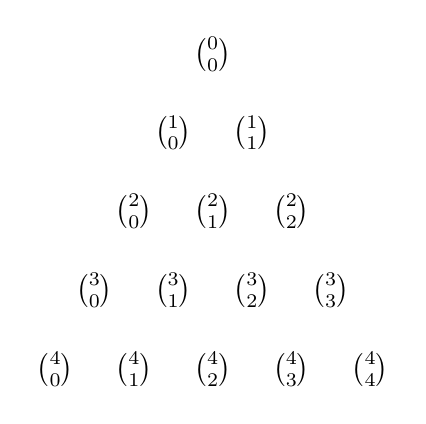
\begin{tikzpicture}
        \foreach \n in {0,...,4} {
            \foreach \k in {0,...,\n} {
                \node at (\k-\n/2,-\n) {$\binom{\n}{\k}$};
            }
        }
    \end{tikzpicture}%
 \end{minipage}%
 \pause % Honestly impressive that this works
 \begin{minipage}{0.5\linewidth}
  \centering
    \begin{tikzpicture}
        \foreach \n in {0,...,4} {
            \foreach \k in {0,...,\n} {
                \node at (\k-\n/2,-\n) {$\binomialCoefficient{\n}{\k}$};
            }
        }
    \end{tikzpicture}%
 \end{minipage}
\end{figure} 
\end{frame}

\begin{frame}{A Pattern in the Triangle}
    \begin{figure}
        \centering
        \includegraphics[scale=1]{images/Pascal8.png}
    \end{figure}
\end{frame}

\begin{frame}{A Pattern in the Triangle}
    \begin{figure}
        \centering
        \includegraphics[scale=1]{images/PascalFib8.png}
    \end{figure}
\end{frame}

% ======================================================
\iffalse
% Remove this and the \fi for induction proof version
% ======================================================
\begin{frame}{Proving the Pattern}
    \underline{\textbf{Claim}}: 
    \[
        \sum_{k = 0}^{n} \binom{n - k}{k} = F_{n + 1}
    \]
    
    \vspace{30pt}
    
    \begin{center}
        We are going to prove this by \underline{\textbf{induction}}
    \end{center} \pause
    
    \underline{\textbf{Base Cases}}: 
    \begin{align*}
        F_0 &= 1                                           & F_1 &= 1 \\
        \sum_{k = 0}^0 \binom{0 - k}{k} &= \binom{0}{0} = 1   & \sum_{k = 0}^k \binom{1 - k}{k} &= \binom{1}{0} + \binom{0}{1} = 1
    \end{align*}
\end{frame}

\begin{frame}{Lemma: A Combinatorial Argument}
    One reason combinatorics is so fascinating is that many proofs can be done without tedious algebra, just using logic and counting. \pause
    
    \vspace{40pt}
    
    \underline{\textbf{Lemma}}:
    \[  
        \binom{n + 1}{k} = \binom{n}{k} + \binom{n}{k - 1}
    \]
\end{frame}

\begin{frame}{Proving the Pattern: Tedious Algebra}
    Assume now that $\sum\limits_{k = 0}^{j} \binom{j - k}{k} = F_{j + 1}$ for $2 \leq j \leq n$.
    \begin{align*}
        \onslide<+->{F_n + F_{n + 1}} &=\action<+->{\sum_{k = 0}^{n - 1} \binom{n - 1 - k}{k} + \sum_{k = 0}^{n} \binom{n - k}{k} = }  \action<+->{\sum_{k = 1}^{n} \binom{n - k}{k - 1} + \sum_{k = 0}^{n} \binom{n - k}{k} \\}
        \onslide<+->{                &= \sum_{k = 1}^{n} \binom{n - k}{k - 1} + \binom{n}{0} + \sum_{k = 1}^{n} \binom{n - k}{k} = } \action<+->{1 + \sum_{k = 1}^n \binom{n - k}{k - 1} + \binom{n - k}{k} \\}
        \onslide<+->{                &= 1 + \sum_{k = 1}^n \binom{n + 1 - k}{k} = } \action<+->{\binom{n + 1- k}{0} + \sum_{k = 1}^n \binom{n + 1 - k}{k} \\}
        \onslide<+->{                &= \sum_{k = 0}^n \binom{n + 1 - k}{k} = } \action<+->{F_{n + 2} \\}
    \end{align*}
\end{frame}
% ======================================================
\fi
% ======================================================

\begin{frame}{Proving the Pattern}
    \underline{\textbf{Claim}}: 
    \[
        \sum_{k = 0}^{\left\lfloor \frac{n}{2} \right\rfloor} \binom{n - k}{k} = F_{n + 1}
    \]
    
    \vspace{30pt}
    
    \begin{center}
        We are going to prove this by a \underline{\textbf{combinatorial argument}}
    \end{center}
    
\end{frame}

\begin{frame}{Staircases}
    \underline{\textbf{Question:}} How many ways are there to climb a staircase going one or two steps at a time?
    \begin{figure}
        \centering
        \includegraphics[scale=0.9]{images/staircase.png}
    \end{figure}
    {\textcolor{white}{invisible text to make the next slide transition smoother}}
\end{frame}

\begin{frame}{Staircases}
    \underline{\textbf{Question:}} How many ways are there to climb a staircase going one or two steps at a time?
    \begin{figure}
        \centering
        \includegraphics[scale=0.9]{images/staircase_red.png}
    \end{figure}
    We can think of this recursively!
\end{frame}

\begin{frame}{Steps to Compute Steps}
    \begin{itemize}
        \item Let the starting step be step $0$. Assuming we are on step $n \geq 2$, how did we get here? \pause
        \begin{itemize}
            \item Either we took a single step from step $n - 1$ \pause
            \item Or we took two steps from step $n - 2$ \pause
        \end{itemize}
        \item Combining the number of ways to get to step $n - 1$ with the number of ways to get to step $n - 2$ yields the number of ways to get to step $n$ \pause
        \item $S_n = S_{n - 1} + S_{n - 2}$ \pause
        \begin{itemize}
            \item How many ways are there to get to step $0$? \textbf{Exactly 1} ($S_0 = 1$) \pause
            \item How many ways are there to get to step $1$? \textbf{Exactly 1} ($S_1 = 1$) \pause
        \end{itemize}
        \item $S_n = F_{n + 1}$
    \end{itemize}
\end{frame}

\begin{frame}{Making Choices}
    \begin{itemize}
        \item There is another angle to the staircase problem \pause
        \item We can just choose which steps to take two steps from, and fill the rest with single steps 
    \end{itemize}
    \begin{figure}
        \centering
        \includegraphics[scale=0.9]{staircase_choose.png}
    \end{figure}
\end{frame}

\begin{frame}{Placing Steps}
    \begin{itemize}
        \item We have to choose where to place our steps of size $2$
        \item If we have $n$ steps, how many ways can we place $k$ steps of size 2? \pause
    \end{itemize}
    \[
        \binom{n - k}{k} \text{ ways}
    \] \pause
    \begin{itemize}
        \item How many possible values of $k$ are there? \pause
    \end{itemize}
    \[
        \left\lfloor \frac{n}{2} \right\rfloor
    \] \pause
    \[
        \text{Thus, } \sum_{k = 0}^{\left\lfloor \frac{n}{2} \right\rfloor} \binom{n - k}{k} = S_n = F_{n + 1}
    \]
\end{frame}

\begin{frame}{}
      \begin{center}
    {\color{sigma@mainblue} \LARGE Questions?}
  \end{center}
\end{frame}

\font\eightss=cmssq8
\font\eightssi=cmssqi8
\newcommand\quoteAuthorDate[3]{\begingroup
  \baselineskip 10pt
  \parfillskip 0pt
  \interlinepenalty 10000 % not needed in example
  \leftskip 0pt plus 40pc minus \parindent
  \let\rm=\eightss
  \let\sl=\eightssi
  \everypar{\sl}#1\par
  \nobreak\smallskip
  \noindent\rm--- #2\unskip\enspace(#3)\par
  \endgroup}
% If someone can figure out how to horizontally center this and make the text bigger that'd be cool
\begin{frame}
    \begin{center}
        \item \quoteAuthorDate{[Combinatorics] has a relation to almost every species of useful knowledge that the mind of man can be employed upon.}{JAMES BERNOULLI, Ars Conjectandi (``The Art of Conjecturing")}{\color{sigma@mainblue} 1713}
    \end{center}
\end{frame}

% Remove this slide if you came up with all the material yourself
\begin{frame}{Bibliography}
    \bibliography{refs}
    \bibliographystyle{alpha}
\end{frame}

\end{document}